%% abtex2-modelo-trabalho-academico.tex, v-1.9.2 laurocesar
%% Copyright 2012-2014 by abnTeX2 group at http://abntex2.googlecode.com/ 
%%
%% This work may be distributed and/or modified under the
%% conditions of the LaTeX Project Public License, either version 1.3
%% of this license or (at your option) any later version.
%% The latest version of this license is in
%%   http://www.latex-project.org/lppl.txt
%% and version 1.3 or later is part of all distributions of LaTeX
%% version 2005/12/01 or later.
%%
%% This work has the LPPL maintenance status `maintained'.
%% 
%% The Current Maintainer of this work is the abnTeX2 team, led
%% by Lauro César Araujo. Further information are available on 
%% http://abntex2.googlecode.com/
%%
%% This work consists of the files abntex2-modelo-trabalho-academico.tex,
%% delo-include-comandos and abntex2-modelo-references.bib
%%

% ------------------------------------------------------------------------
% ------------------------------------------------------------------------
% abnTeX2: Modelo de trabalho Academico (tese de doutorado, dissertacao de
% mestrado e trabalhos monograficos em geral) em conformidade com 
% ABNT NBR 14724:2011: Informacao e documentacao - Trabalhos academicos -
% Apresentacao
% ------------------------------------------------------------------------
% ------------------------------------------------------------------------

\documentclass[
	% -- opções da classe memoir --
	12pt,				% tamanho da fonte
	openright,			% capítulos começam em pág ímpar (insere página vazia caso preciso)
	twoside,			% para impressão em verso e anverso. Oposto a oneside
	a4paper,			% tamanho do papel. 
	% -- opções da classe abntex2 --
	%chapter=TITLE,		% títulos de capítulos convertidos em letras maiúsculas
	%section=TITLE,		% títulos de seções convertidos em letras maiúsculas
	%subsection=TITLE,	% títulos de subseções convertidos em letras maiúsculas
	%subsubsection=TITLE,% títulos de subsubseções convertidos em letras maiúsculas
	% -- opções do pacote babel --
	english,			% idioma adicional para hifenização
	brazil				% o último idioma é o principal do documento
	]{abntex2ufop} % classe abntex2ufop para escrita de trabalhos academicos

% ---
% Pacotes básicos 
% ---
\usepackage{lmodern}			% Usa a fonte Latin Modern			
\usepackage[T1]{fontenc}		% Selecao de codigos de fonte.
\usepackage[utf8]{inputenc}		% Codificacao do documento (conversão automática dos acentos)
\usepackage{lastpage}			% Usado pela Ficha catalográfica
\usepackage{indentfirst}		% Indenta o primeiro parágrafo de cada seção.
\usepackage{color}				% Controle das cores
\usepackage{graphicx}			% Inclusão de gráficos
\usepackage{microtype} 			% para melhorias de justificação
\usepackage{supertabular}       % tabela na capa do dosudo apt-get install texlive texlive-latex3cumento
% ---
		
% ---
% Pacotes adicionais, usados apenas no âmbito do Modelo Canônico do abnteX2 - pode ser removido

% ---
% Pacotes adicionais, usados no anexo do modelo de folha de identificação
% ---
\usepackage{multicol}
\usepackage{multirow}
\usepackage{lipsum}				% para geração de dummy text
% ---

% ---
% Pacotes de citações
% ---
\usepackage[brazilian,hyperpageref]{backref}	 % Paginas com as citações na bibliografia
\usepackage[alf]{abntex2cite}	% Citações padrão ABNT 6023

% --- 
% CONFIGURAÇÕES DE PACOTES
% --- 

% ---
% Configurações do pacote backref
% Usado sem a opção hyperpageref de backref
\renewcommand{\backrefpagesname}{Citado na(s) página(s):~}
% Texto padrão antes do número das páginas
\renewcommand{\backref}{}
% Define os textos da citação
\renewcommand*{\backrefalt}[4]{
	\ifcase #1 %
		Nenhuma citação no texto.%
	\or
		Citado na página #2.%
	\else
		Citado #1 vezes nas páginas #2.%
	\fi}%
% ---

% ---
% Informações de dados para CAPA e FOLHA DE ROSTO
% ---
\titulo{Sistema modular integrado para monitoramento de água com solução IoT.}
\autor{Camilo Esteves Mendes de Avelar}
\local{Ouro Preto}
\data{2018}
\orientador{Filipe Augusto Santos Rocha}
\coorientador{}
\instituicao{Universidade Federal de Ouro Preto - UFOP - Escola de Minas - Colegiado do curso de Engenharia de Controle e Automa{\c c}{\~a}o - CECAU}
\tipotrabalho{Monografia de Gradua{\c c}{\~a}o em Engenharia de Controle e Automa{\c c}{\~a}o }
% O preambulo deve conter o tipo do trabalho, o objetivo, 
% o nome da instituição e a área de concentração 
\preambulo{Monografia apresentada ao Curso de Engenharia de Controle e Automa{\c c}{\~a}o da Universidade Federal de Ouro Preto como parte dos requisitos para a obten{\c c}{\~a}o do Grau de Engenheiro de Controle e Automa{\c c}{\~a}o.}
% ---


% ---
% Configurações de aparência do PDF final

% alterando o aspecto da cor azul
\definecolor{blue}{RGB}{41,5,195}

% informações do PDF
\makeatletter
\hypersetup{
     	%pagebackref=true,
		pdftitle={\@title}, 
		pdfauthor={\@author},
    	pdfsubject={\imprimirpreambulo},
	    pdfcreator={LaTeX with abnTeX2},
		pdfkeywords={abnt}{latex}{abntex}{abntex2}{trabalho acadêmico}, 
		colorlinks=true,       		% false: boxed links; true: colored links
    	linkcolor=blue,          	% color of internal links
    	citecolor=blue,        		% color of links to bibliography
    	filecolor=magenta,      		% color of file links
		urlcolor=blue,
		bookmarksdepth=4
}
\makeatother
% --- 

% --- 
% Espaçamentos entre linhas e parágrafos 
% --- 

% O tamanho do parágrafo é dado por:
\setlength{\parindent}{1.3cm}

% Controle do espaçamento entre um parágrafo e outro:
\setlength{\parskip}{0.2cm}  % tente também \onelineskip

% ---
% compila o indice
% ---
\makeindex
% ---

% ----
% Início do documento
% ----
\begin{document}

% Retira espaço extra obsoleto entre as frases.
\frenchspacing 

% ----------------------------------------------------------
% ELEMENTOS PRÉ-TEXTUAIS
% ----------------------------------------------------------
% \pretextual

% ---
% Capa
% ---
\imprimircapa
% ---

% ---
% Folha de rosto
% (o * indica que haverá a ficha bibliográfica)
% ---
\imprimirfolhaderosto*
% ---


% ---
% Inserir a ficha bibliografica
% ---

% Isto é um exemplo de Ficha Catalográfica, ou ``Dados internacionais de
% catalogação-na-publicação''. 
% Porém, a biblioteca da sua universidade lhe fornecerá um PDF
% com a ficha catalográfica definitiva após a defesa do trabalho. Quando estiver
% com o documento, salve-o como PDF no diretório do seu projeto e substitua todo
% o conteúdo de implementação deste arquivo pelo comando abaixo que está comentado 
% (nao se esqueça de comentar o antigo ambiente de ficha catalográfica):
%
% \begin{fichacatalografica}
%     \includepdf{fig_ficha_catalografica.pdf}
% \end{fichacatalografica}
%
%
% Ou, você poderá também ler os dados da ficha e adicionar no póprio código
% como as palavras-chave, CDU e dimensões do trabalho: 
\begin{fichacatalografica}
	\vspace*{\fill}					% Posição vertical
	\hrule							% Linha horizontal
	\begin{center}					% Minipage Centralizado
	\begin{minipage}[c]{12.5cm}		% Largura
	
	\imprimirautor
	
	\hspace{0.5cm} \imprimirtitulo  / \imprimirautor. --
	\imprimirlocal, \imprimirdata-
	
	\hspace{0.5cm} \pageref{LastPage} p. : il. (algumas color.) ; 30 cm.\\
	
	\hspace{0.5cm} \imprimirorientadorRotulo~\imprimirorientador\\
	
	\hspace{0.5cm}
	\parbox[t]{\textwidth}{\imprimirtipotrabalho~--~\imprimirinstituicao,
	\imprimirdata.}\\
	
	\hspace{0.5cm}
		1. Palavra-chave1.
		2. Palavra-chave2.
		I. Orientador.
		II. Universidade xxx.
		III. Faculdade de xxx.
		IV. Título\\ 			
	
	\hspace{8.75cm} CDU 02:141:005.7\\
	
	\end{minipage}
	\end{center}
	\hrule
\end{fichacatalografica}
% ---

% ---
% Inserir folha de aprovação
% ---

% Isto é um exemplo de Folha de aprovação, elemento obrigatório da NBR
% 14724/2011 (seção 4.2.1.3). Você pode utilizar este modelo até a aprovação % do trabalho. Após isso, substitua todo o conteúdo deste arquivo por uma % imagem da página assinada pela banca com o comando abaixo:
%
% \includepdf{folhadeaprovacao_final.pdf}
%
\begin{folhadeaprovacao}
% 
   Monografia defendida e aprovada, em $XX$ de $XX$ de \imprimirdata, pela comiss{\~a}o avaliadora constitu{\'i}da pelos professores:
   \vspace*{\fill}
   \assinatura{\textbf{\imprimirorientador} \\ Orientador} 
   \vspace*{\fill}
   \assinatura{\textbf{ \\ Convidado}}
   \vspace*{\fill}
   \assinatura{\textbf{ \\ Convidado}}
   \vspace*{\fill}
   %\assinatura{\textbf{Professor} \\ Convidado 3}
  % \vspace*{\fill}
   %\assinatura{\textbf{Professor} \\ Convidado 4}
  % \vspace*{\fill}
      
   \begin{center}
    \vspace*{0.5cm}
    {\large\imprimirlocal}, {\large\imprimirdata}
    \vspace*{1cm}
  \end{center}
  
\end{folhadeaprovacao}
% ---

% ---
% Dedicatória
% ---
% \begin{dedicatoria}
%   \vspace*{\fill}
%   \flushright
%   \noindent
%   \textit{ Este trabalho é dedicado às crianças adultas que,\\
%   quando pequenas, sonharam em se tornar cientistas.} \vspace*{\fill}
% \end{dedicatoria}
% ---

% ---
% Agradecimentos
% ---
\begin{agradecimentos}
\noindent Os agradecimentos depois de pronto.

\end{agradecimentos}
% ---
% ---
% Epígrafe
% ---
%\begin{epigrafe}
%    \vspace*{\fill}
	%\begin{flushright}
	%	\textit{``Matéria é a parte acidental.'' (Oliver Lodge)}
	%\end{flushright}
%\end{epigrafe}
% ---

% ---
% RESUMOS
% ---

% resumo em português
\setlength{\absparsep}{18pt} % ajusta o espaçamento dos parágrafos do resumo
\begin{resumo}
 \noindent 

 \textbf{Palavras-chaves}: iot, sistema, monitoramento, esp8266
\end{resumo}

% resumo em inglês
% \begin{resumo}[Abstract]
%  \begin{otherlanguage*}{english}

% \noindent This is the english abstract.

%   \vspace{\onelineskip}
 
%   \noindent 
%   \textbf{Key-words}: latex. abntex. text editoration.
%  \end{otherlanguage*}
% \end{resumo}

% resumo em francês 
%\begin{resumo}[Résumé]
% \begin{otherlanguage*}{french}
%    Il s'agit d'un résumé en français.
% 
%   \textbf{Mots-clés}: latex. abntex. publication de textes.
% \end{otherlanguage*}
%\end{resumo}
%
%% resumo em espanhol
%\begin{resumo}[Resumen]
% \begin{otherlanguage*}{spanish}
%   Este es el resumen en español.
%  
%   \textbf{Palabras clave}: latex. abntex. publicación de textos.
% \end{otherlanguage*}
%\end{resumo}
%% ---

% ---
% inserir lista de ilustrações
% ---
\pdfbookmark[0]{\listfigurename}{lof}
\listoffigures*
\cleardoublepage
% ---

% ---
% inserir lista de tabelas
% ---
%\pdfbookmark[0]{\listtablename}{lot}
%\listoftables*
%\cleardoublepage
% ---

% ---
% inserir lista de abreviaturas e siglas
% ---
%\begin{siglas}
 % \item[ABNT] Associação Brasileira de Normas Técnicas
 % \item[abnTeX] ABsurdas Normas para TeX
%\end{siglas}
% ---

% ---
% inserir lista de símbolos
% ---
%\begin{simbolos}
  % \item[$ \Gamma $] Letra grega Gama
  % \item[$ \Lambda $] Lambda
  % \item[$ \zeta $] Letra grega minúscula zeta
  % \item[$ \in $] Pertence
%\end{simbolos}
% ---

% ---
% inserir o sumario
% ---
\pdfbookmark[0]{\contentsname}{toc}
\tableofcontents*
\cleardoublepage
% ---



% ----------------------------------------------------------
% ELEMENTOS TEXTUAIS
% ----------------------------------------------------------
\textual
% ----------------------------------------------------------
% PARTE
% ----------------------------------------------------------
%\part{Preparação da pesquisa}
% ----------------------------------------------------------
%
% ---
% Modelo de capitulo com a introducao, objetivos e estrutura do texto
% ---
% ----------------------------------------------------------
% Introdução (exemplo de capítulo sem numeração, mas presente no Sumário)
% ----------------------------------------------------------
\chapter[Introdução]{Introdução}
%\addcontentsline{toc}{chapter}{Introdução}
% ----------------------------------------------------------

Cerca de 70\% da superfície do planeta é coberta por água, quase toda salgada e, portanto, imprópria para o consumo humano. Apenas 2,5\% desse total é potável e a maior parte das reservas (cerca de 80\%) está concentrada em geleiras nas calotas polares. 
Essa quantidade reduzida de recursos aliada ao contínuo e intenso crescimento demográfico ao longo dos anos, o desenvolvimento industrial e, por consequência, o aumento do consumo de água nas grandes cidades, tem sido um dos principais temas de discussões e palestras de conscientização por todo o mundo. \cite{aguaconsumo}

Pesquisas indicam que, em poucas décadas, as reservas de água doce do planeta não serão suficientes para suprir as necessidades humanas caso os níveis de consumo não sejam controlados desde já \cite{Diarias2007}. A escassez deste recurso essencial à vida acarretará em problemas de ordem política, econômica e sanitária, podendo até originar conflitos similares aos causados pelo domínio do petróleo.

A economia de água é um assunto recorrente que há muito deixou de ser restrito às regiões áridas e desérticas com baixa disponibilidade de água per capita. Isto faz com que governos e organizações de todo o mundo estejam com atenções voltadas para a criação de políticas de consumo sustentável, programas de educação ambiental, alternativas e soluções para a redução e controle do uso da água. \cite{ferreirasistema}.

A fim de evitar consequências como a escassez da água, o consumo
responsável encabeça a lista de medidas a serem tomadas por se tratar de uma atitude factível a todas as pessoas. \cite{Diarias2007}. Recentemente, avanços em recursos computacionais e tecnologias de eletrônicos permitiram a criação do paradigma do IoT (Internet of Things ou Internet das Coisas). \citeauthor{Perumal2016} (\citeyear{Perumal2016}) descrevem a Internet das Coisas como sendo um método para conectar coisas em torno do ambiente e realizar um certo tipo de troca de mensagem entre eles, integrando-os.

O IoT representa uma rede mundial de objetos interconectados e unicamente endereçados. Esta conectividade entre sensores e atuadores permite o compartilhamento de informações entre plataformas através de um \textit{framework} unificado, desenvolvendo uma comum capacidade de criar aplicações inovadoras. Isto é possível devido a sensores, analise da dados e representação de informações através de Computação em Nuvem como o \textit{framework} unificado. \cite{RisteskaStojkoska2017}

Uma das grandes influências do IoT é no campo do monitoramento do ambiente em que vivemos, sistemas de alarmes e análise de dados ambientais \cite{Perumal2016}. %Este trabalho propõe a elaboração, planejamento e implementação de um sistema de baixo custo para monitoramento e economia de água no uso de chuveiros elétricos residenciais.

O desenvolvimento de tecnologias de infraestrutura no início do século XX, como as redes de água e esgoto, gás encanado e eletricidade fizeram com que a residências se conectassem com o meio externo, tornando-se um nó de uma grande rede \cite{forty2007objetos}. Com o advento da Internet, essa ligação se acentuou, permitindo ainda mais conectividade. \cite{VarelaDeSouza} 

Segundo \citeauthor{VarelaDeSouza} (\citeyear{VarelaDeSouza}), a palavra "Domótica" resulta da junção da palavra latina
“Domus”, que significa casa, com “Robótica”, que pode ser entendido como controle automatizado de algum processo ou equipamento. Seu uso pode trazer significativas vantagens a seus usuários como a otimização e gestão de recursos, praticidade, segurança, controle e monitoramento remoto dos dispositivos automatizados.



\section{Objetivos}

O objetivo deste trabalho é desenvolver um sistema modular, de baixo custo, baseado em microsserviços e no paradigma do IoT, para monitoramento e controle de consumo de água de chuveiros elétricos através da integração entre microprocessadores, microcontroladores, sensores e atuadores. 

O sistema será capaz de armazenar e exibir dados vindos dos sensores de fluxo de água em sistemas remotos, conectados através da rede Wi-Fi, além de comandar um atuador para interromper o fornecimento da água.

Será criado também um sistema que emulará os dados provindos do sensor, atuador e teclado utilizados.

\subsection{Objetivos específicos}

\begin{itemize}
	\item Armazenar dados para levantamentos estatísticos;
	\item Implementar o sistema de identificação e controle de usuários;
	\item Implementar o sistema de interface;
	\item Implementar o sistema de atuação;
	\item Implementar o sistema de emulação de dados;
	\item Integrar todos os sistemas a fim de garantir as funcionalidades do projeto;
	\item Monitorar em ambiente online dos parâmetros do sistema;
\end{itemize}

\section{Justificativas e Relev{\^a}ncia}
%
Segundo \citeauthor{AlvesDaSilva} (\citeyear{AlvesDaSilva}), o crescente consumo de água
tem feito do uso consciente uma necessidade primordial. Essa prática deve ser considerada parte de uma atividade mais abrangente que é o uso racional da água, incluindo também, o controle de perdas e a redução do consumo de água.

Ao passar dos anos, os desperdícios da água utilizada atingem níveis nunca imaginados \cite{rebouccas2003agua}. Ao combinar as técnicas de eletrônica e automação, será possível otimizar o monitoramento do gasto de água em residências e prédios, visando coletar dados para diminuir este tipo de desperdício. Este trabalho se justifica pela urgente necessidade de controle do uso da água em todas as esferas da sociedade. 
%
\section{Organização do trabalho}

O presente trabalho está organizado em 5 Capítulos. No Capitulo 1, encontra-se a apresentação do problema e suas possíveis soluções, além de apresentar os objetivos propostos.

O Capítulo 2 consiste na revisão sobre os hardwares e softwares utilizados no projeto, encontram-se as definições e explicações dos mesmos.

No Capítulo 3 é apresentado a estrutura geral do sistema, a metodologia em que foi construído. Explica-se também as etapas do desenvolvimento e códigos implementados.

O Capítulo 4 trata dos experimentos realizados no sistema e seus resultados.

No Capítulo 5 são abordadas as considerações finais do trabalho e os possíveis trabalhos futuros.
% ---
% Capitulo com exemplos de comandos inseridos de arquivo externo 
% ---
\include{capitulos/capitulo-abntex2-modelo-include-comandos}
% ---
% ----------------------------------------------------------
% PARTE
% ----------------------------------------------------------
%\part{Referenciais teóricos}
% ----------------------------------------------------------
% ---
% Capitulo de revisão de literatura
% ---
\chapter{Revisão Bibliográfica}
% ---

% ---
\section{Microcontroladores e Microprocessadores}
% ---

Para uma melhor eficiência no processamento de dados, na década de 70
começaram a ser utilizados microprocessadores em computadores \cite{martins2005sistemas}. 

Os microprocessadores são componentes dedicados ao processamento de informações com
capacidade de cálculos matemáticos e endereçamento de memória externa \cite{chase2007sistemas}.

\subsection{ESP8266}

O ESP8266 é um circuito totalmente integrado, com interfaces de I\\O digitais e analógicas e, ainda, interface WiFi, com um processador de 32 bits, capaz de executar a 160 MHz.

Os módulos baseados no microcontrolador ESP8266 representam um grande avanço na relação de preço-recursos e podem ser um componente muito interessante para suluções IoT.\cite {de2017internet}

\begin{figure}[htbp]
		\centering
		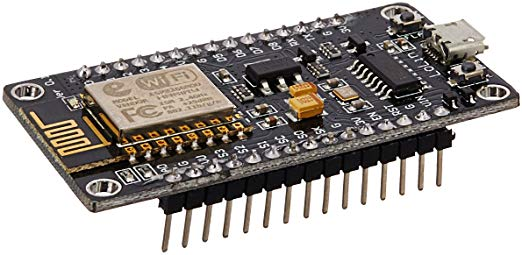
\includegraphics[scale=0.5]{figuras/esp8266_.jpg}
		\caption{ESP8266}
		\label{fig:09}
\end{figure}

\subsection{RaspberryPi}

Raspberry Pi é um minicomputador criado pela
Raspberry Pi Foundation com o objetivo de estimular o
ensino da ciência da computação nas escolas e
universidades. Apesar de o Raspberry Pi possuir o
hardware em uma única placa eletrônica de tamanho
reduzido, seu potencial de processamento é significativo.
O Raspberry Pi pode ser usado em diversos projetos
tecnológicos, como experimentos remotos nos quais sua
função é ser um Micro servidor web.\cite{crotti2013raspberrypi}

\begin{figure}[htbp]
		\centering
		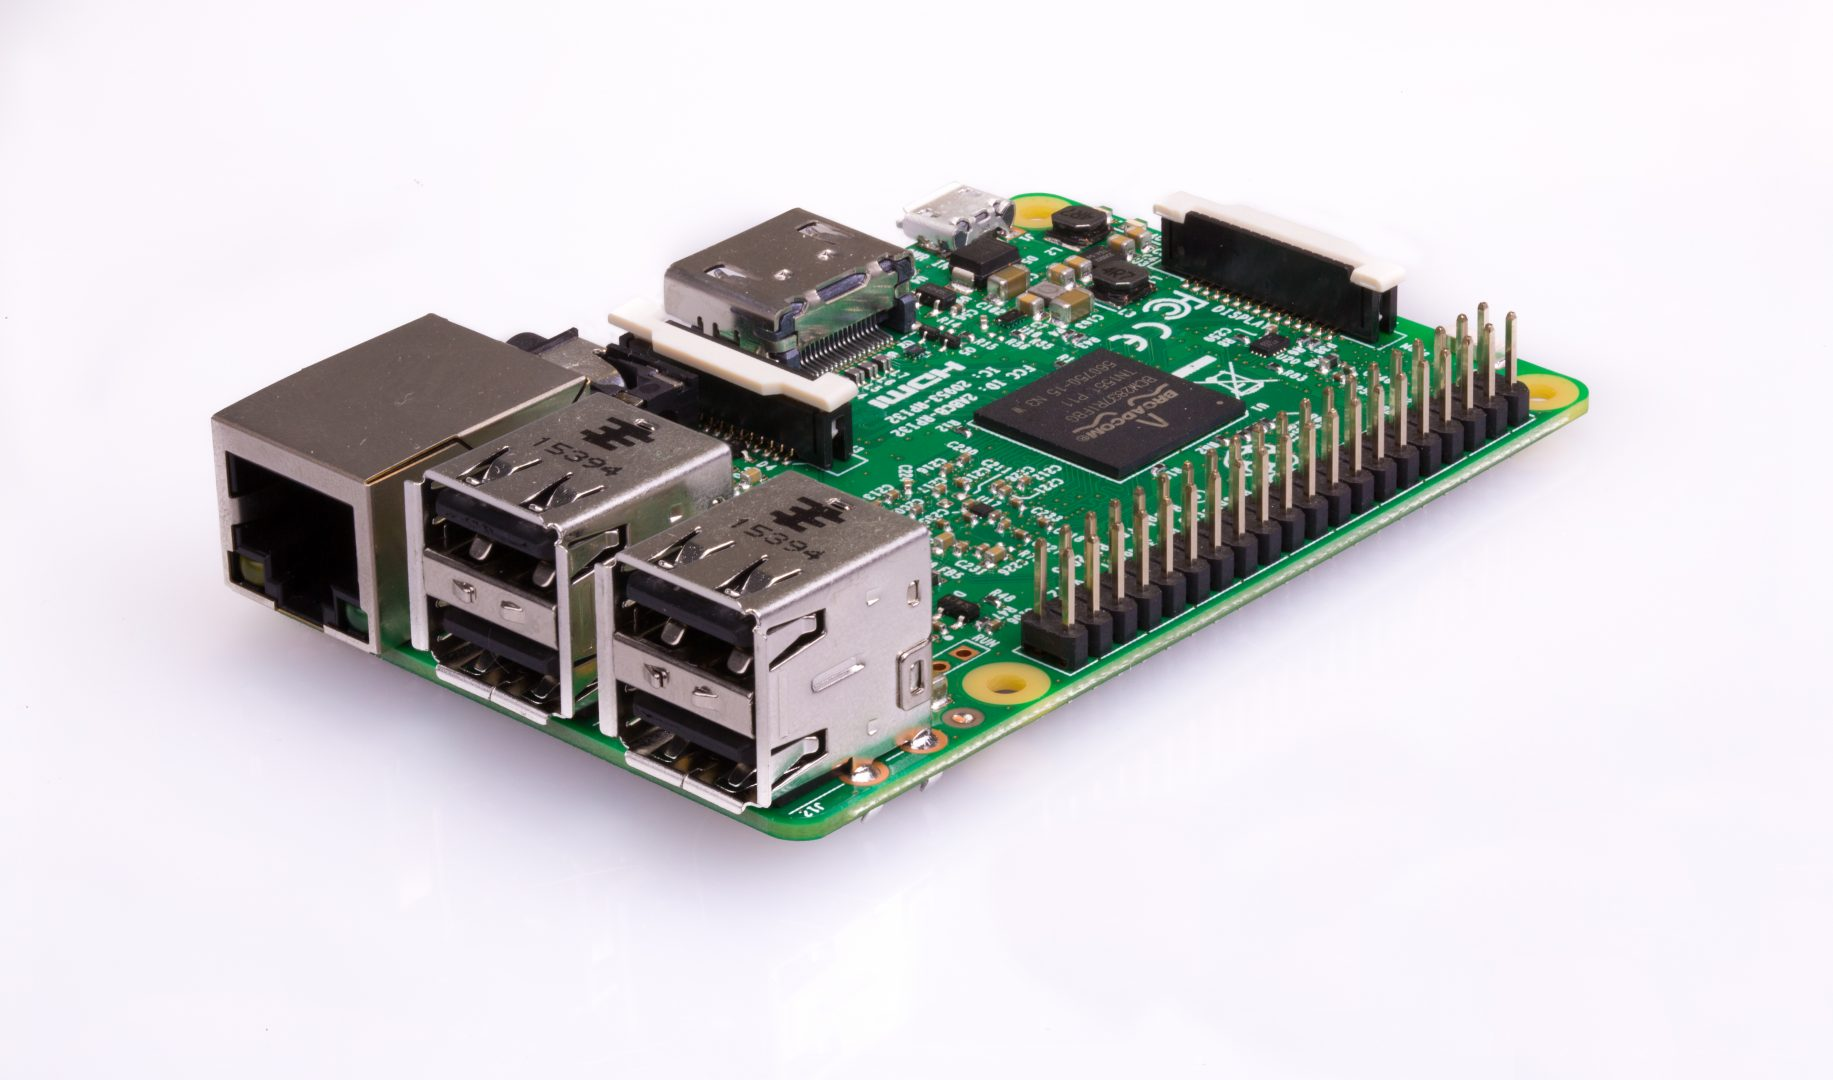
\includegraphics[scale=0.2]{figuras/raspberrypi.jpg}
		\caption{RaspberryPi}
		\label{fig:09}
\end{figure}

\section{Sensor de fluxo YF-S201}

São sensores do tipo turbina que medem a quantidade de líquido que passa pela tubulação, girando uma turbina que
gera pulsos de onda quadrada através de um sensor de efeito Hall\cite{roque2018sistema} O
sensor usa esse efeito para enviar um sinal PWM,e através desse pulso é possível mensurar a quantidade de água que passa pelo cata-vento no interior do sensor, cada pulso mede aproximadamente 2,25 mm.\cite{ms2017automaccao}

\begin{figure}[htbp]
		\centering
		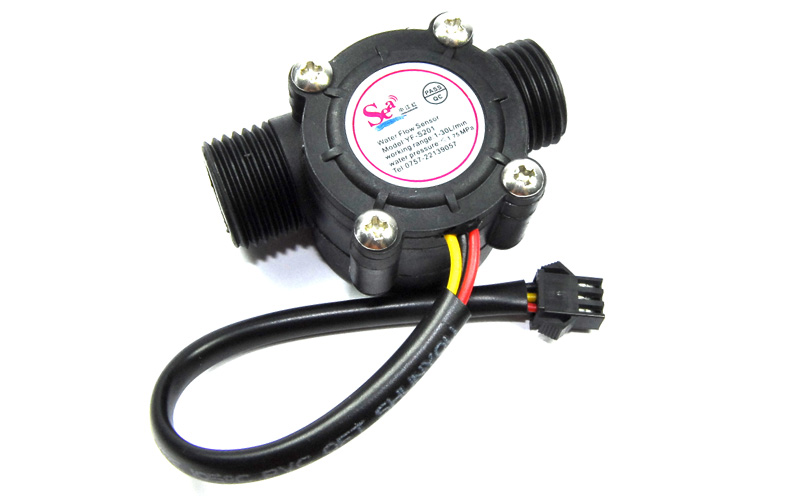
\includegraphics[scale=0.3]{figuras/yf-s201.jpg}
		\caption{Sensor de fluxo de água YF-S201}
		\label{sensor}
\end{figure}
% ----------------------------------------------------------
% PARTE
% ----------------------------------------------------------
%\part{Resultados}
% ----------------------------------------------------------
% ---
% primeiro capitulo de Resultados
\chapter{Experimentos e Resultados}

Neste Capítulo encontram-se os experimentos realizados com os sistemas devidamente implementados e configurados. Discutiremos os resultados obtidos, testando os sistemas com todas as suas funcionalidades.

\section{Manipulação de usuários}

O microsserviço de usuários utiliza a porta 3001. Para utiliza-lo e testa-lo, devemos utilizar esta porta juntamente com os \textit{endpoints} disponíveis (Seção \ref{sec:usuarios}). Aqui realizaremos as consultas em todos estes \textit{endpoints} e discutiremos os resultados obtidos.

Para criar um usuário devemos consumir\footnote{O termo "consumir um \textit{endpoint}"\  significa enviar informações para o \textit{endpoint}, esperando algum retorno, de sucesso ou falha.} o \textit{endpoint} http://localhost:3001/usuario/cadastrar passando os parâmetros via \textit{POST} no formato \textit{JSON}\footnote{Javascript Object Notation (JSON), é um formato compacto de troca de dados simples e rápida entre sistema}, como na Figura \ref{fig:cadastro}.

A resposta deste \textit{endpoint} pode ser conferida na Figura \ref{fig:cadastro} e, para garantir que o usuário foi incluído no banco de dados, podemos observar a Figura \ref{fig:cadastro}.

\begin{figure}[htbp]
	\centering
	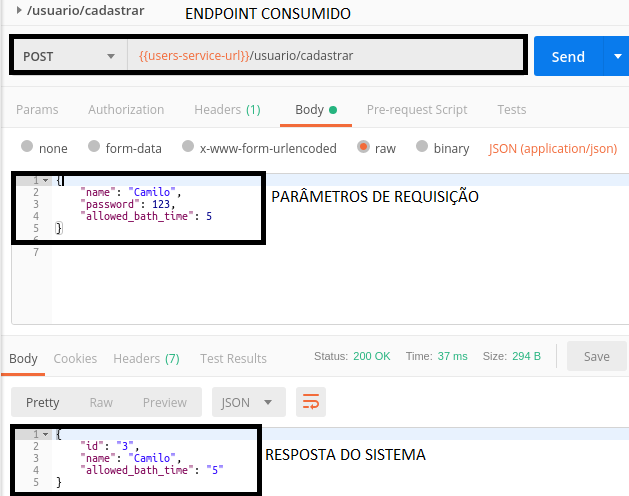
\includegraphics[width=0.7\linewidth]{figuras/postman/cadastro.png}
	\caption{Cadastro de usuários}
	\label{fig:cadastro}
\end{figure}

\clearpage

O \textit{endpoint} http://localhost:3001/usuario/editar-tempo deve ser consumido para editar o tempo máximo de banho de um usuário (Figura \ref{fig:tempo}). Para editar a senha do usuário, deve-se consumir o \textit{endpoint} http://localhost:3001/usuario/editar-senha (Figura \ref{fig:senha}).

\begin{figure}[htbp]
	\centering
	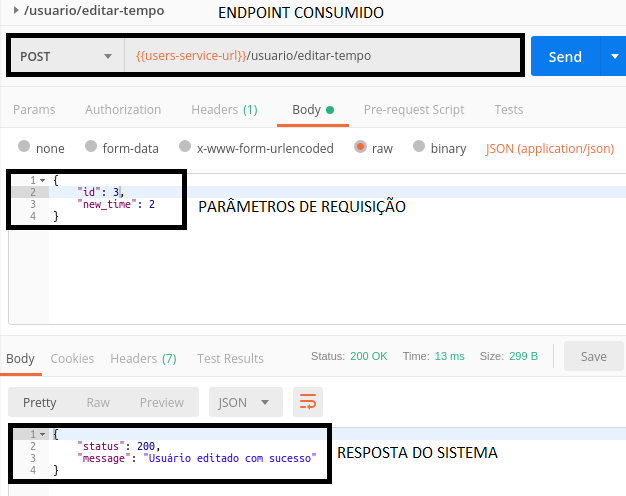
\includegraphics[width=0.7\linewidth]{figuras/postman/time.png}
	\caption{Edição de tempo permitido do usuário}
	\label{fig:tempo}
\end{figure}

\begin{figure}[htbp]
	\centering
	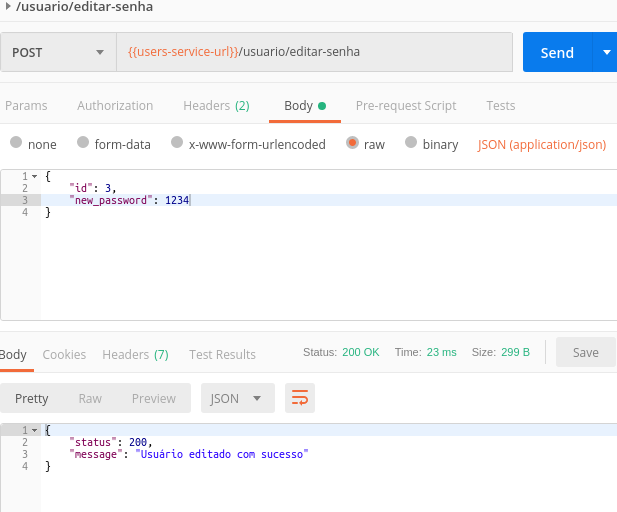
\includegraphics[width=0.7\linewidth]{figuras/postman/password.png}
	\caption{Edição de senha do usuário}
	\label{fig:senha}
\end{figure}

Conseguimos cadastrar um banho ao consumir o \textit{endpoint} http://localhost:3001/banho via \textit{POST} com os parâmetros e resposta mostrados na Figura \ref{fig:banho}.

\begin{figure}[htbp]
	\centering
	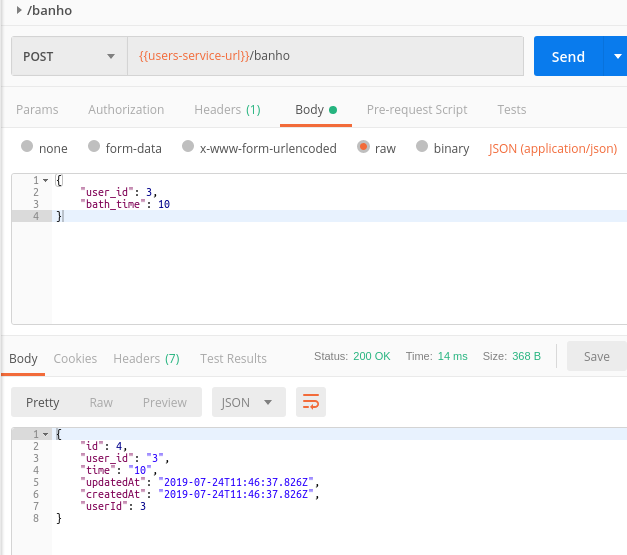
\includegraphics[width=0.7\linewidth]{figuras/postman/bathsinclude.png}
	\caption{Adicionando banhos ao usuário}
	\label{fig:banho}
\end{figure}

Para recuperar as informações de um usuário, basta consumir o \textit{endpoint} \break http://localhost:3001/usuario/idDoUsuario, com o método \textit{GET}, obtendo o resultado da Figura \ref{fig:usuario}.

\begin{figure}[htbp]
	\centering
	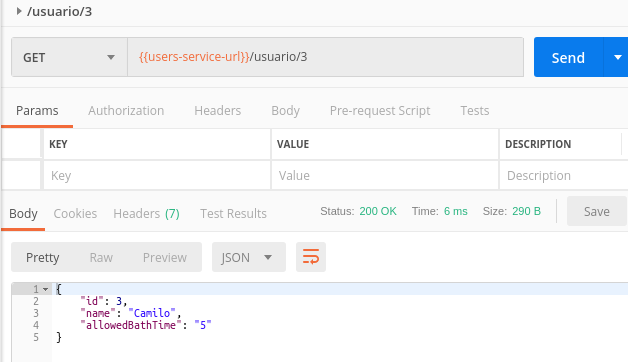
\includegraphics[width=0.7\linewidth]{figuras/postman/getuser.png}
	\caption{Recuperar dados do usuário}
	\label{fig:usuario}
\end{figure}

Conseguimos as informações de todos os banhos dos usuários consumindo o \textit{endpoint} http://localhost:3001/banho/idDoUsuario, via \textit{GET}, e conseguiremos o resultado exibido na Figura \ref{fig:banhos}.

\begin{figure}[htbp]
	\centering
	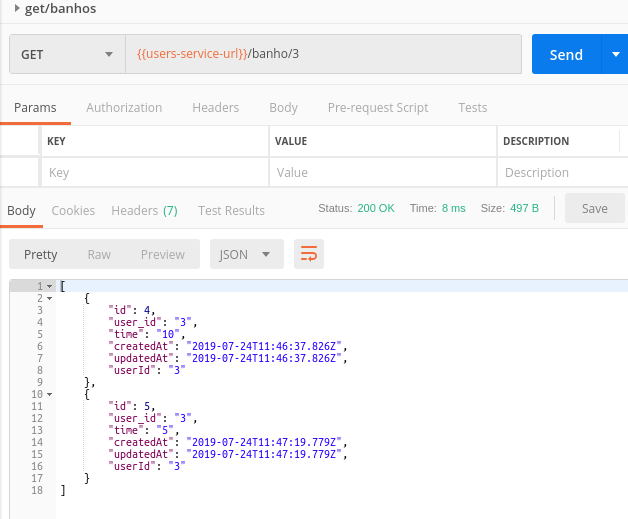
\includegraphics[width=0.7\linewidth]{figuras/postman/getbanhos.png}
	\caption{Recuperar dados de banhos do usuário}
	\label{fig:banhos}
\end{figure}

Finalmente, podemos autenticar os usuários enviando via \textit{POST} os parâmetros para o \textit{endpoint} http://localhost:3001/usuario/autorizar, obtendo como resposta a Figura \ref{fig:allowedtrue}, para usuário autenticado, e Figura \ref{fig:allowedfalse}, para usuário não autenticado, caso a senha esteja errada.

\begin{figure}[htbp]
	\centering
	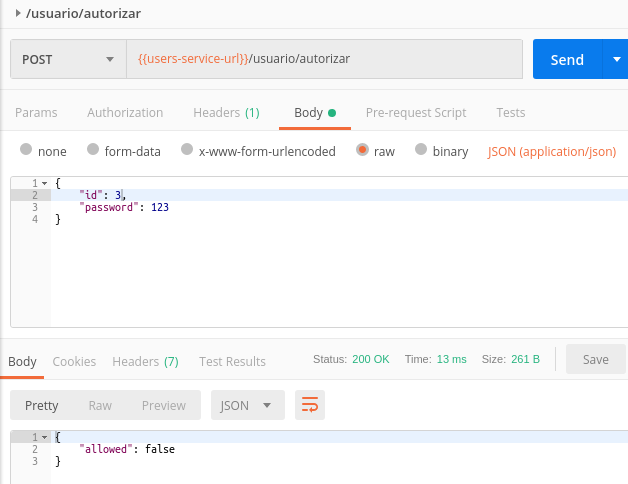
\includegraphics[width=0.7\linewidth]{figuras/postman/allowedfalse.png}
	\caption{Exemplo de usuário não autorizado}
	\label{fig:allowedfalse}
\end{figure}

\begin{figure}[htbp]
	\centering
	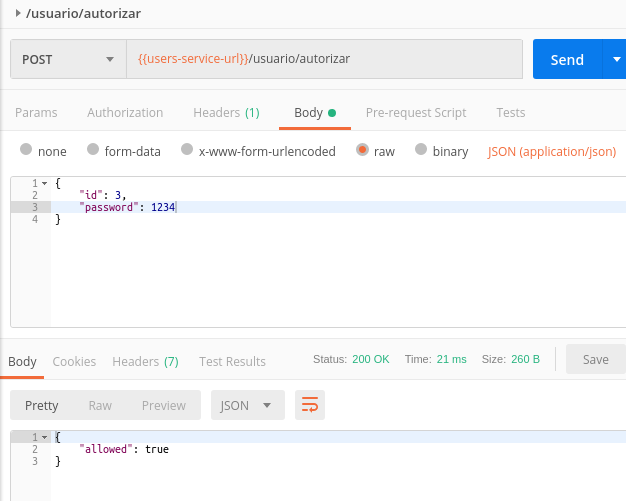
\includegraphics[width=0.7\linewidth]{figuras/postman/allowedtrue.png}
	\caption{Exemplo de usuário autorizado}
	\label{fig:allowedtrue}
\end{figure}

\section{Visualização via Grafana}

Ao autenticar um usuário, o atuador é ativado e o sensor YF-S201 inicia a medição do fluxo, que é automaticamente enviado para o InfluxDB, podendo ser visualizado via Grafana. Os gráficos do grafana podem ser acessados via http://localhost:3003, como na Figura \ref{fig:grafanahome}.

Pode ser observado na Figura \ref{fig:grafana-graph} um gráfico do fluxo medido pelo sensor no horário de 09h30m até 09h35m, por dois usuários diferentes.

\begin{figure}[htbp]
	\centering
	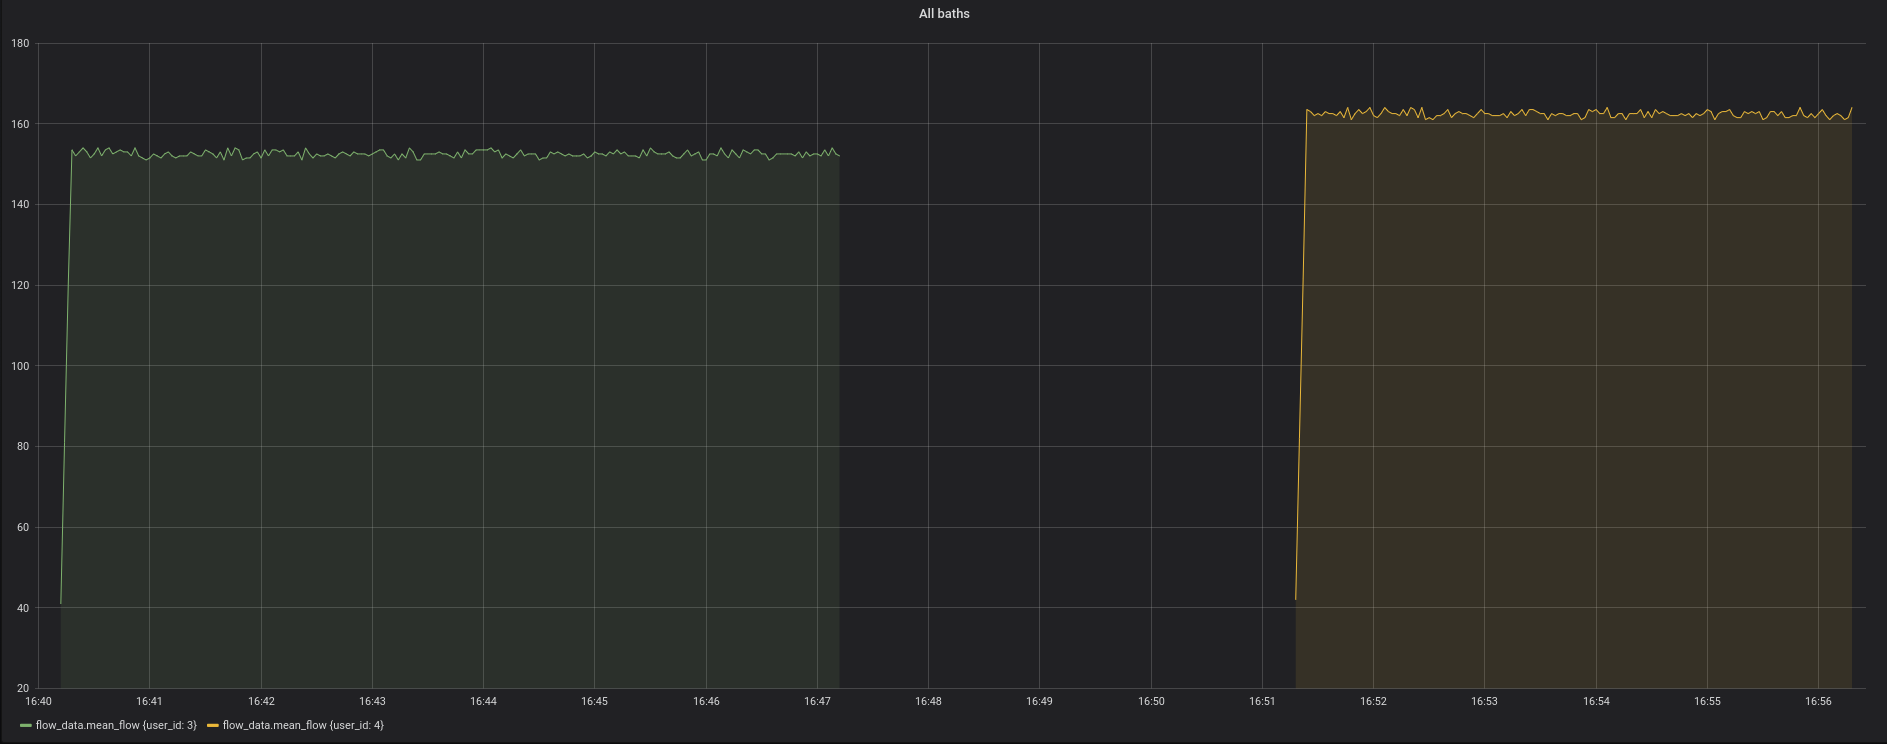
\includegraphics[width=1\linewidth]{figuras/grafanagraph.png}
	\caption{Exemplo do gráfico no Grafana para usuários diferentes}
	\label{fig:grafana-graph}
\end{figure}

\section{Estado do atuador via HomeAssistant}

O HomeAssistant é acessado via http://localhost:8123. Ao acessar o link, observamos os estado dos sensores dos usuários cadastrado na Figura \ref{fig:homeassistant-off}, que encontram-se em estado desligado. Ao digitar corretamente a senha, o estado do sensor muda para ligado, como observado na Figura \ref{fig:homeassistant-on}.

\begin{figure}[htbp]
	\centering
	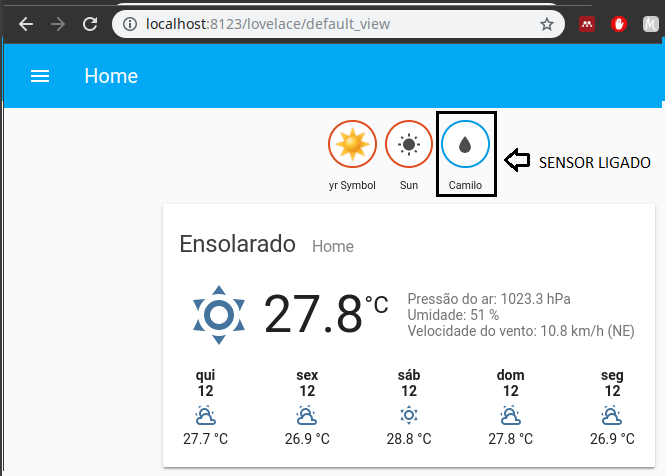
\includegraphics[width=0.6\linewidth]{figuras/homeassistanton.png}
	\caption{Exemplo do sensor no HomeAssistant quando ligado}
	\label{fig:homeassistant-on}
\end{figure}

\begin{figure}[htbp]
	\centering
	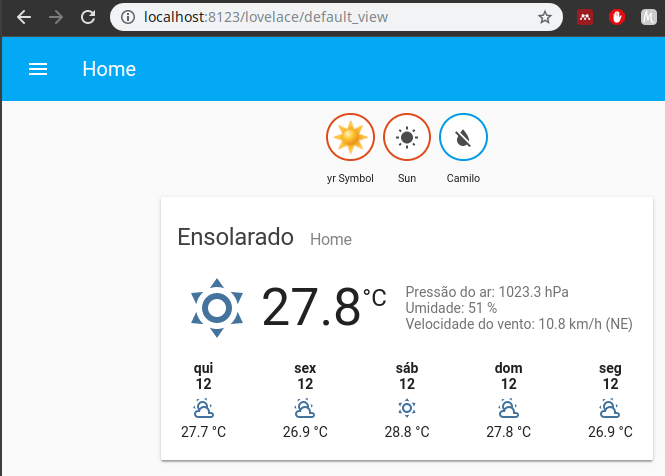
\includegraphics[width=0.6\linewidth]{figuras/homeassistantoff.png}
	\caption{Exemplo do sensor no HomeAssistant quando desligado}
	\label{fig:homeassistant-off}
\end{figure}

Ao cadastrar um usuário, o seu sensor é inserido no HomeAssistant automaticamente (Figura \ref{fig:homeassistant-new}).

\begin{figure}[htbp]
	\centering
	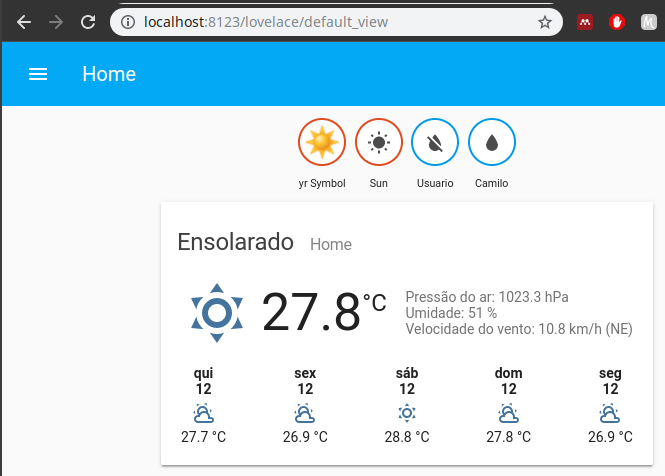
\includegraphics[width=1\linewidth]{figuras/homeassistantnewuser.png}
	\caption{Exemplo de um novo sensor quando um novo usuário é cadastrado}
	\label{fig:homeassistant-new}
\end{figure}



% ----------------------------------------------------------
% Finaliza a parte no bookmark do PDF
% para que se inicie o bookmark na raiz
% e adiciona espaço de parte no Sumário
% ----------------------------------------------------------
%\phantompart
% ---
% Insere arquivo de Considerações Finais ou Conclusões
% ---
\chapter{Considerações Finais}

Este trabalho propõe um sistema capaz de monitorar remotamente a utilização da água em uma residência. Os sistemas de monitoramento propostos foram implementados. Como mostrado, a implementação é capaz de cadastrar, editar e autorizar usuários. Monitorar o fluxo de água e o tempo de banhos com gráficos e estados de sensores em tempo real remotamente, comportando-se como deveria.

O sistema físico não foi criado, devido à necessidade de proteção extra, como caixas resistentes à água e vapores para garantir o seu funcionamento e durabilidade.

Ao final do desenvolvimento do projeto e dos resultados apresentado, pode-se concluir que o sistema é eficaz no monitoramento remoto auxiliando o usuário na gestão da utilização de água em chuveiros. Podendo ser um grande aliado na redução do consumo de água em toda a residência, se implementado em outros setores, como torneiras ou tanques.

Para trabalhos futuros, pode-se realizar a implementação física em chuveiros com sensores e proteção mais robustos que sejam resistentes ao vapor de água presente ao se tomar banho. 

Seria interessante a implementação de mais sistemas de monitoramento utilizando outros sensores realizando a integração com HomeAssistant implementando apenas pequenas modificações e configurações extras. O sistema foi arquitetado e construído com o intuito de facilitar esta inclusão de sensores e reutilização.
% ----------------------------------------------------------
% ELEMENTOS PÓS-TEXTUAIS
% ----------------------------------------------------------
\postextual
% ----------------------------------------------------------
% ----------------------------------------------------------
% Referências
% ----------------------------------------------------------
\bibliography{abntex2-modelo-references}
% ----------------------------------------------------------
% Glossário
% ----------------------------------------------------------
%
% Consulte o manual da classe abntex2 para orientações sobre o glossário.
%
%\glossary

% ----------------------------------------------------------
% Apêndices
% ----------------------------------------------------------
%(Lembre-se: Apendices são de autoria do próprio autor do texto. 
% Anexos são elementos de autorias de outros, que o autor do texto julga interessante apresentar)
% ---
% Inicia os apêndices: 
% ---
\begin{apendicesenv}

% Imprime uma página indicando o início dos apêndices
\partapendices
% ---
% Insere arquivo com os apendices A e B
\chapter{Código sistema de usuários} \label{ap:users}

Neste apêndice encontram-se algumas partes importantes do código do Sistema de Usuários. O código inteiro pode ser baixado no \textit{link}: \url{https://github.com/CamiloAvelar/user-service}

\begin{lstlisting}[caption=Exemplo do código do \textit{interactor} de criação do usuário]
import Interactor from './interactor';
import usersRep from '../repositories/users.rep';
import bcrypt from 'bcrypt';
import config from './../config/config';

class CreateUserBs extends Interactor {
	constructor(){
		super();
	}
	
	async execute({ name, password, allowedBathTime }) {
	
		if (!allowedBathTime) {
			allowedBathTime = 10;
		}
	
		const hash = await bcrypt.hash(password.toString(), config.bcrypt.saltRounds);
	
		const user = await usersRep.createUser({ name, password: hash, allowedBathTime });
		
		if(!user) {
			throw 'Nao foi possivel criar o usuario!';
		}
		
		const response = {
			id: user.user_id,
			name: user.user.name,
			allowed_bath_time: user.allowed_bath_time,
		};
		
		return response;
	}
}

export default CreateUserBs;
\end{lstlisting}

\begin{lstlisting}[caption=Exemplo do código do \textit{interactor} de edição de senha de usuários]
import Interactor from './interactor';
import usersRep from '../repositories/users.rep';
import bcrypt from 'bcrypt';
import config from './../config/config';

class EditPasswordBs extends Interactor {
	constructor(){
		super();
	}
	
	async execute({ id, new_password }) {
	
		const hash = await bcrypt.hash(new_password.toString(), config.bcrypt.saltRounds);
		
		const editedUser = await usersRep.editPassword({ id, password: hash });
		
		const response = editedUser[0] === 1 ? {
			status: 200,
			message: 'Usuario editado com sucesso'
		} : 
		{
			status: 500,
			message: 'Erro ao editar usuario'
		};
		
		return response;
	}
}
\end{lstlisting}

\newpage

\begin{lstlisting}[caption=Exemplo do código do \textit{interactor} de edição de tempo de banho dos usuários]
import Interactor from './interactor';
import usersRep from '../repositories/users.rep';

class EditUserTimeBs extends Interactor {
	constructor() {
		super();
	}
	
	async execute({ id, new_time }) {
	
		const editedUser = await usersRep.editUserTime({ id, new_time });
		
		const response = editedUser[0] === 1 ? {
			status: 200,
			message: 'Usuario editado com sucesso'
		} : 
		{
			status: 500,
			message: 'Erro ao editar usuario'
		};
		
		return response;
	
	}
}
\end{lstlisting}

\newpage

\begin{lstlisting}[caption=Exemplo do código do \textit{interactor} de autorização de usuários]
import Interactor from './interactor';
import usersRep from '../repositories/users.rep';
import bcrypt from 'bcrypt';

class AuthorizeUserBs extends Interactor {
	constructor(){
		super();
	}
	
	async execute({ id, pass }) {
		const user = await usersRep.getUser({ id });
		
		if(!user) {
			throw {error: 'Usuario nao encontrado'};
		}
		
		const match = await bcrypt.compare(pass.toString(), user.password);
		
		return {
			allowed: match
		};
	}
}
\end{lstlisting}

\newpage

\begin{lstlisting}[caption=Exemplo do código do \textit{interactor} de cadastro de banhos]
import Interactor from './interactor';
import bathsRep from '../repositories/baths.rep';

class BathsBs extends Interactor {
	constructor(){
		super();
	}
	
	async execute({ user_id, bath_time }) {
	
		const bath = await bathsRep.createBath({
			user_id,
			bath_time
		});
		
		if(!bath) {
			throw 'Nao foi possivel cadastrar o banho';
		}
		
		return bath;
		}
		
		async getBaths ({ user_id }) {
		
		const baths = await bathsRep.getBaths({
			user_id,
		});
		
		return baths;
	}
}

export default BathsBs;
\end{lstlisting}

\newpage

\begin{lstlisting}[caption=Exemplo do código do \textit{interactor} para recuperar informações dos usuários]
import Interactor from './interactor';
import usersRep from '../repositories/users.rep';

class GetUserBs extends Interactor{
	constructor(){
		super();
	}
	
	async execute({ id }) {
	const user = await usersRep.getUser({ id });
	
	if(!user) {
		throw {error: 'Nao foi possivel localizar o usuario!'};
	}
	
	const response = {
		id: user.id,
		name: user.name,
		allowedBathTime: user.user_setting.allowed_bath_time
	};
	
	return response;
	}
}
\end{lstlisting}

%\begin{figure}[htbp]
%	\centering
%	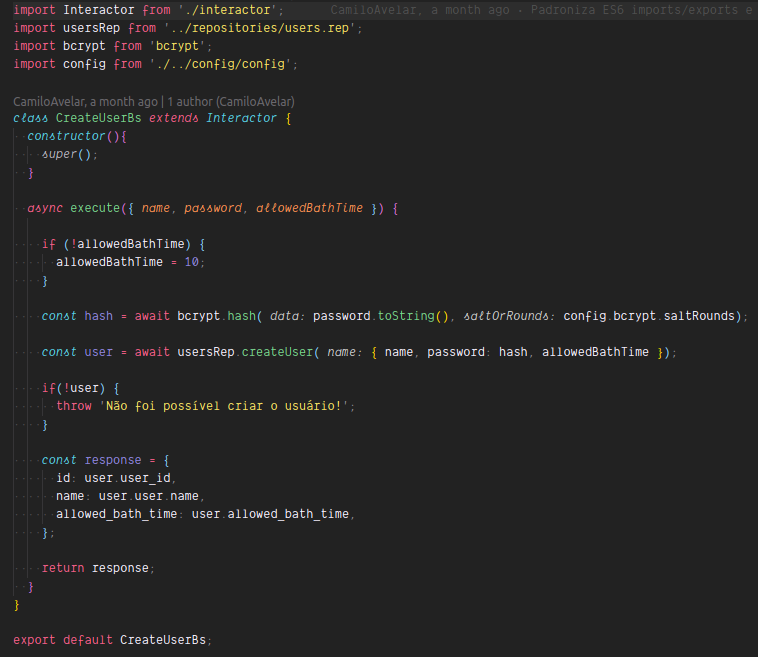
\includegraphics[width=1\linewidth]{figuras/userservice/createuser.png}
%	\caption{Código para criar usuário}
%	\label{fig:createuser}
%\end{figure}
%
%\begin{figure}[htbp]
%	\centering
%	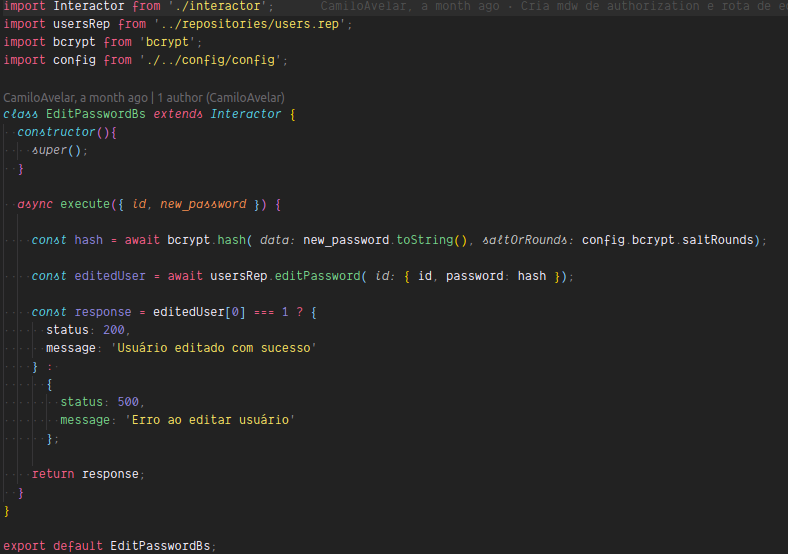
\includegraphics[width=1\linewidth]{figuras/userservice/editpassword.png}
%	\caption{Código para editar senha do usuário}
%	\label{fig:editpass}
%\end{figure}
%
%\begin{figure}[htbp]
%	\centering
%	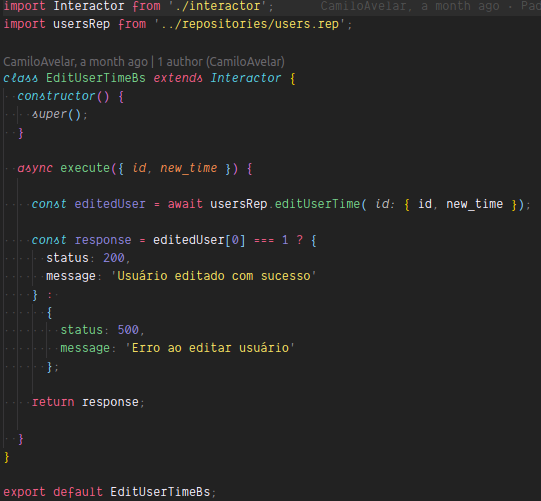
\includegraphics[width=1\linewidth]{figuras/userservice/edittime.png}
%	\caption{Código para editar tempo do usuário}
%	\label{fig:edittime}
%\end{figure}
%
%\begin{figure}[htbp]
%	\centering
%	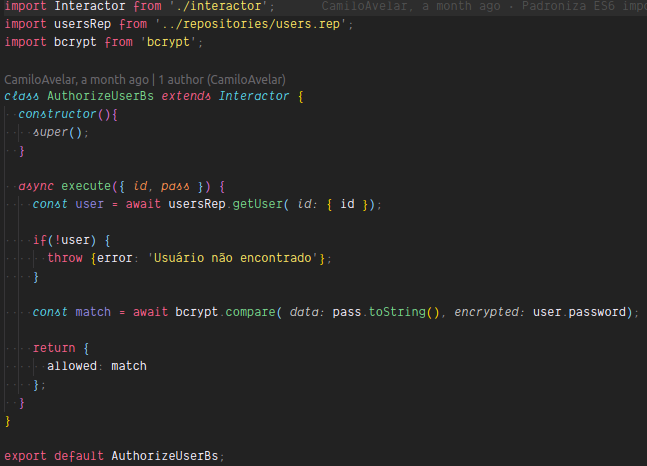
\includegraphics[width=1\linewidth]{figuras/userservice/authorizeuser.png}
%	\caption{Código para autorizar usuário}
%	\label{fig:autorizar}
%\end{figure}
%
%\begin{figure}[htbp]
%	\centering
%	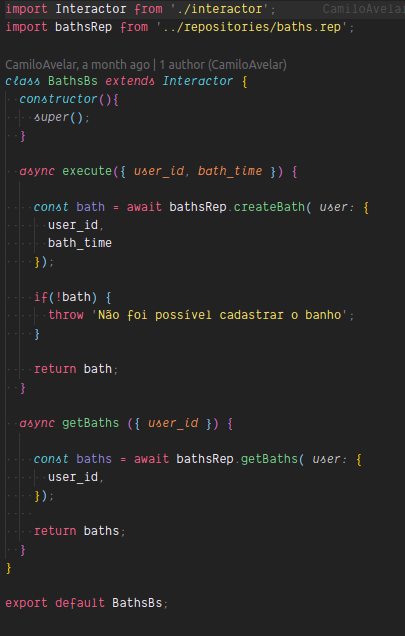
\includegraphics[width=1\linewidth]{figuras/userservice/baths.png}
%	\caption{Código para cadastrar banho do usuário}
%	\label{fig:cadastra-banho}
%\end{figure}
%
%\begin{figure}[htbp]
%	\centering
%	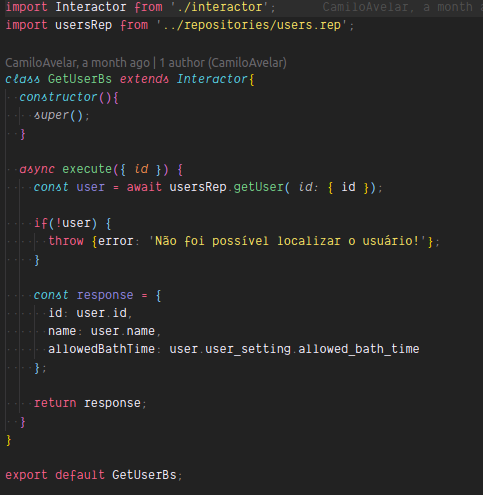
\includegraphics[width=1\linewidth]{figuras/userservice/getuser.png}
%	\caption{Código para recuperar usuários}
%	\label{fig:getuser}
%\end{figure}

\chapter{Código sistema de comunicação MQTT} \label{ap:mqtt}

Neste apêndice encontram-se algumas partes importantes do código do Sistema de comunicação. O código inteiro pode ser baixado no \textit{link}: \url{https://github.com/CamiloAvelar/mqtt-logger-service}

\begin{lstlisting}[caption=Exemplo do código de comunicação MQTT]
const mqtt = require('mqtt');
const EventEmitter = require('events');


class MqttHandler extends EventEmitter {
	constructor() {
		super();
		this.mqttClient = null;
		this.host = 'mqtt://mosquitto';
		this.username = 'mqtt_user'; // mqtt credentials if these are needed to connect
		this.password = '100200300';
	}
	
	
	connect() {
		const self = this;
		this.mqttClient = mqtt.connect(this.host, { username: this.username, password: this.password });
		
		this.mqttClient.on('error', (err) => {
			console.log(err);
			this.mqttClient.end();
		});
		
		this.mqttClient.on('connect', () => {
			console.log(`mqtt client connected to ${this.host}`);
		});
		
		this.mqttClient.on('close', () => {
			console.log(`mqtt client disconnected`);
		});
		
		this.mqttClient.on('message', (topic, message) => {
			const builtMessage = {
				topic,
				message: message.toString()
			};
		
			self.emit('messageReceived', builtMessage);
		})
	}
	
	subscribe(topic) {
		this.mqttClient.subscribe(topic, {qos: 0});
	}
	
	sendMessage(message, topic) {
		this.mqttClient.publish(topic, message);
	}
}

module.exports = MqttHandler;
\end{lstlisting}

\begin{lstlisting}[caption=Exemplo do código responsável por lidar com informações do tempo de banho]
const requestService = require('./requestService');

class timeHandler {
	constructor(mqttClient) {
		this.mqttClient = mqttClient;
		this.allowedTime;
		this.interval;
		this.nowDate;
		this.endDate;
		this.userId;
	}
	
	countTime(allowedTime, id) {
		this.userId = id;
		this.allowedTime = allowedTime;
		this.nowDate = new Date();
		
		this.interval = setInterval(() => {
		this.mqttClient.sendMessage('stop', 'actuator');
		this.clearBathInterval();
		}, this.allowedTime);
	}
	
	async endTime() {
		this.clearBathInterval();
		this.endDate = new Date();
		
		const bathTime = this.endDate - this.nowDate;
		
		console.log('BATHTIME>>>', bathTime);
		await this._requestUserService(bathTime);
	}
	
	clearBathInterval(){
		clearInterval(this.interval);
	}
	
	async _requestUserService(time) {
		const requestOptions = {
			type: 'POST',
			endpoint: 'banho',
			body: {
			user_id: this.userId,
			bath_time: time
			},
		};
		
		return await requestService.userRequest(requestOptions);
	}
}

module.exports = timeHandler;
\end{lstlisting}

\newpage

\begin{lstlisting}[caption=Exemplo do código que lida com a comunicação com o InfluxDB]
const requestService = require('./requestService');

class KeysHandler {
	constructor(mqttClient) {
		this.keyBuffer = '';
		this.working = false;
		this.gettingPassword = false;
		this.userId;
		this.mqttClient = mqttClient;
	}
	
	async handle(message) {
		if(message === '*') {
			this.working = !this.working;
			this.gettingPassword = false;
			return;
		}
	
		if((this.working || this.gettingPassword) && message !== '#') {
			this.keyBuffer += message;
		}
		
		if(message === '#') {
			this.working = false;
			try {
				const response = await this._requestUserService();
				console.log(response);
				this.gettingPassword ? (response.allowed ? this.mqttClient.sendMessage('start', 'actuator') : console.log('NAO AUTORIZADO')) : 
				this.mqttClient.sendMessage(JSON.stringify(response), 'user');
				this.gettingPassword = !this.gettingPassword;
			} catch (err) {
				console.log(err.message)
			} finally {
				this.keyBuffer = '';
			}
		}
	}
	
	async _requestUserService() {
		const requestOptions = this.gettingPassword ? {
			type: 'POST',
			endpoint: `usuario/autorizar`,
			body:{
				id: this.userId,
				password: this.keyBuffer
			},
			}: {
				type: 'GET',
				endpoint: `usuario/${this.keyBuffer}`,
			body: null,
		};
		
		return requestService.userRequest(requestOptions)
		.then((response) => {
			this.userId = this.gettingPassword ? this.userId : response.id;
			return response
		}).catch(err => {throw err});
	}
}

module.exports = KeysHandler;
\end{lstlisting}

%\begin{figure}[htbp]
%	\centering
%	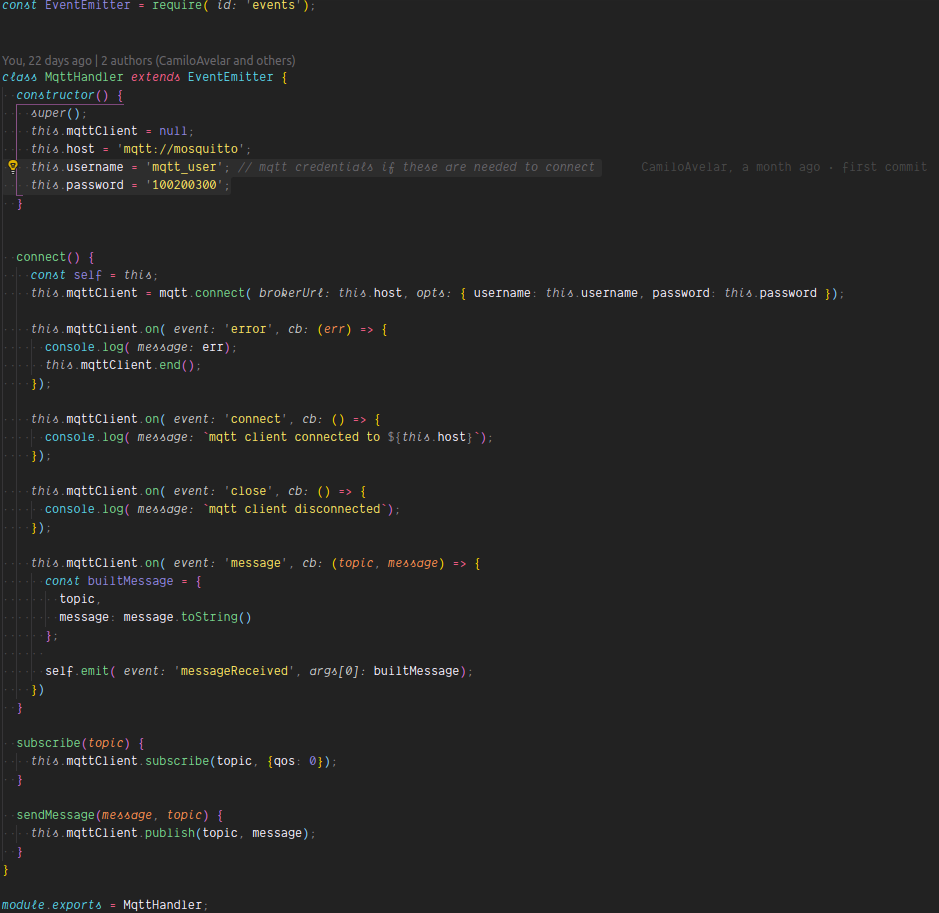
\includegraphics[width=1\linewidth]{figuras/mqttlogger/mqtt.png}
%	\caption{Código para comunicação mqtt}
%	\label{fig:mqtt}
%\end{figure}
%
%\begin{figure}[htbp]
%	\centering
%	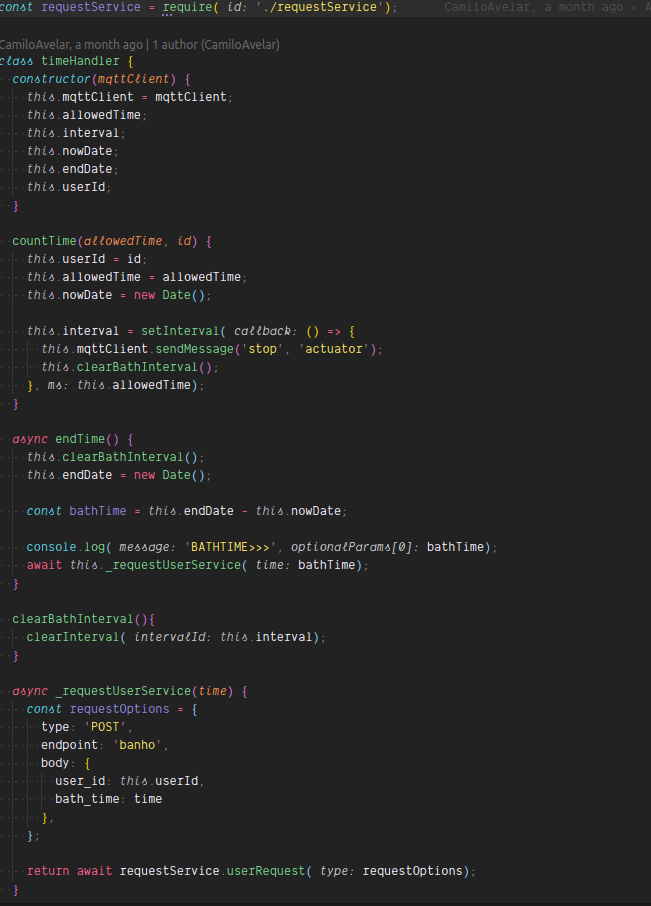
\includegraphics[width=1\linewidth]{figuras/mqttlogger/time.png}
%	\caption{Código que lida com o tempo do banho}
%	\label{fig:time}
%\end{figure}
%
%\begin{figure}[htbp]
%	\centering
%	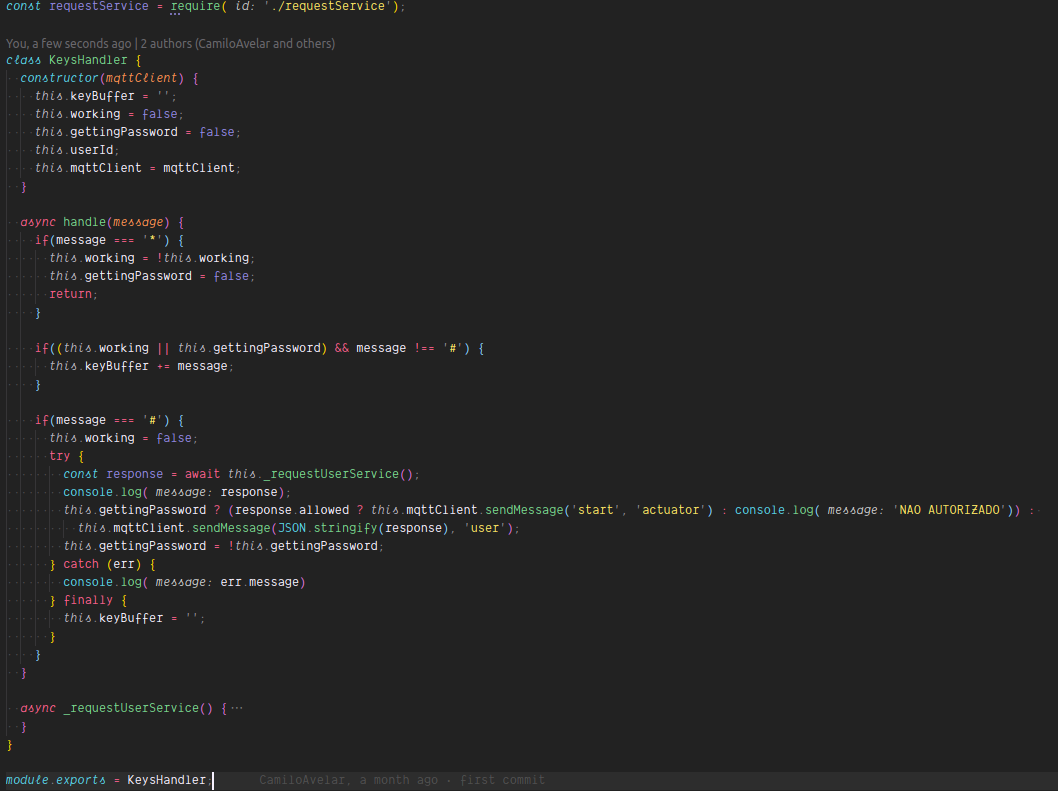
\includegraphics[width=1\linewidth]{figuras/mqttlogger/keystopic.png}
%	\caption{Código que lida com as teclas apertadas no teclado numérico}
%	\label{fig:keys}
%\end{figure}
%
%\begin{figure}[htbp]
%	\centering
%	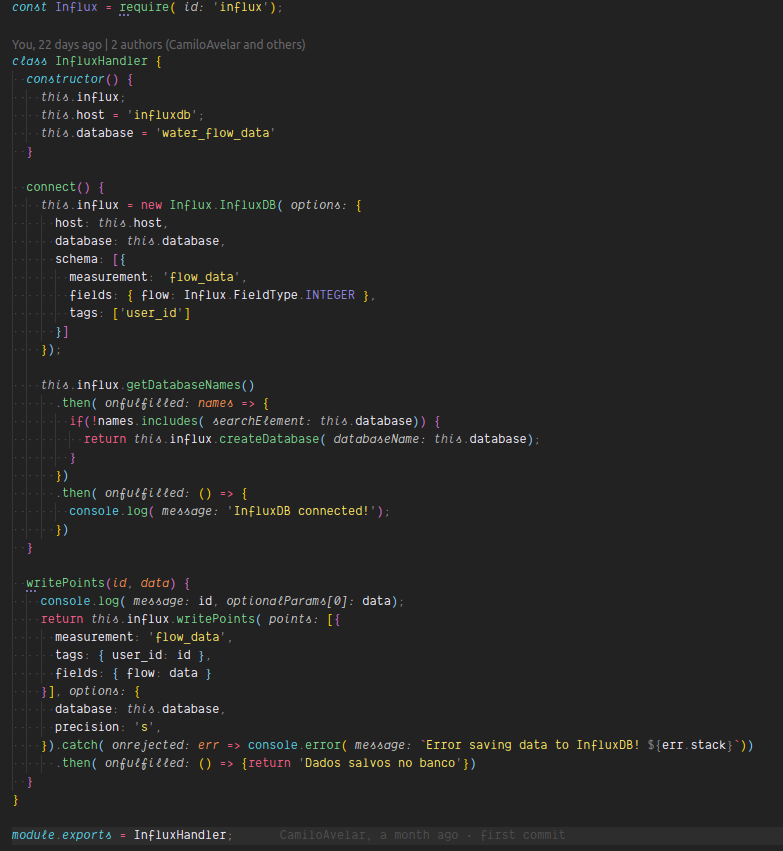
\includegraphics[width=1\linewidth]{figuras/mqttlogger/influx.png}
%	\caption{Código que lida com a comunicação com o InfluxDB}
%	\label{fig:influx}
%\end{figure}

%\chapter{Docker-compose.yml}
%
%\begin{lstlisting}[language=Python]
%version: "3.5"
%
%services:
%	user:
%		build: ./user-service
%		command: gulp
%		depends_on:
%			- postgres
%		volumes:
%			- ./user-service:/app
%		ports:
%			- "3001:3001"
%		networks:
%			- default
%
%	mqtt-logger:
%		build: ./mqtt-logger
%		command: npm start
%		depends_on:
%			- mosquitto
%		volumes:
%			- ./mqtt-logger:/app
%		ports:
%			- "3002:3002"
%
%	postgres:
%		image: postgres
%		restart: always
%		environment:
%		POSTGRES_USER: pi
%		POSTGRES_PASSWORD: 100200300
%		POSTGRES_DB: postgres
%		CONFIGS: "listen_addresses:'*'"
%		volumes:
%			- ./postgres/data:/var/lib/postgresql/data
%		expose:
%			- "5432"
%		ports:
%			- "5432:5432"
%		networks:
%			- default
%
%	migration:
%		image: src_user:latest
%		command: ["./wait-for-it/wait-for-it.sh", "postgres:5432", "--", "npm", "run", "migrate"]
%		links:
%			- postgres
%		depends_on:
%			- postgres
%
%	homeassistant:
%		container_name: homeassistant
%		restart: unless-stopped
%		image: homeassistant/home-assistant
%		volumes:
%			- ./homeassistant:/config
%		depends_on:
%			- mosquitto
%		network_mode: host
%		privileged: true
%		expose:
%			- "8123"
%		ports:
%			- "8123:8123"
%
%	influxdb:
%		image: influxdb:latest
%		container_name: influxdb
%		restart: always
%		ports:
%			- "8083:8083"
%			- "8086:8086"
%			- "8090:8090"
%		volumes:
%			# Data persistency
%			# sudo mkdir -p /srv/docker/influxdb/data
%			- ./influxdb/data:/var/lib/influxdb
%
%	grafana:
%		image: grafana/grafana
%		container_name: grafana
%		restart: always
%		ports:
%			- "3003:3000"
%		links:
%			- influxdb
%		volumes:
%			# Data persistency
%			# sudo mkdir -p /srv/docker/grafana/data; chown 472:472 /srv/docker/grafana/data
%			- ./grafana/data:/var/lib/grafana
%	
%	mosquitto:
%		image: eclipse-mosquitto
%		hostname: mosquitto
%		container_name: mosquitto
%		restart: always
%		user: 1883:1883
%		expose:
%			- "1883"
%			- "9001"
%		ports:
%			- "1883:1883"
%			- "9001:9001"
%		volumes:
%			- ./mosquitto/config:/mosquitto/config
%			# sudo chown 1883:1884 /mosquitto/logs
%			- ./mosquitto/logs:/mosquitto/logs
%		networks:
%			- default
%		networks:
%		default:
%		driver: bridge
%		ipam:
%		config:
%			- subnet: 172.18.1.0/24
%\end{lstlisting}
\end{apendicesenv}
% ---

% ----------------------------------------------------------
% Anexos
% ----------------------------------------------------------
%(Lembre-se: Apendices são de autoria do próprio autor do texto. 
% Anexos são elementos de autorias de outros, que o autor do texto julga interessante apresentar)
% ---
% Inicia os anexos
% ---
\begin{anexosenv}

% Imprime uma página indicando o início dos anexos
\partanexos

% ---
% Insere arquivo com os anexos 1, 2 e 3
\include{capitulos/capitulo-anexos-1-2-3}
% ---
\end{anexosenv}

%---------------------------------------------------------------------
% INDICE REMISSIVO
%---------------------------------------------------------------------
%\phantompart
\printindex
%---------------------------------------------------------------------

\end{document}
